\documentclass[a4paper,12pt]{book}
\usepackage[utf8]{inputenc}
\usepackage{pscyr}          % Нормальные шрифты
\usepackage[russian]{babel} %
\usepackage{graphicx}
\usepackage[left=2cm,right=2cm,top=2cm,bottom=2cm,bindingoffset=0cm]{geometry}
\usepackage{wrapfig}   % обтекаемые текстом блоки
\usepackage{soulutf8}  % выделение текста
\usepackage{xcolor}    % выделение цветом
\usepackage{array}
\usepackage{booktabs}
\usepackage{multirow,bigdelim}
\usepackage{hhline}
\usepackage{tabularx}
\usepackage{hyperref}
\usepackage{amsmath,amssymb}
\usepackage{nccboxes}
\usepackage{mathtext}
\usepackage{floatflt}

\hypersetup{pdftitle={Электромагнитные переходные процессы}}  % метаданные PDF
\hypersetup{pdfauthor={Сергей Александрович Ульянов}}
\hypersetup{pdfcreator={LaTeX}}
\hypersetup{pdfproducer={http://ulianov.net}}


%\hypersetup{ pdfborder={0 0 0}} % чтобы ссылки не выделялись

%\usepackage[dvips]{graphicx}
%\graphicspath{{pic/}}

\begin{document}

\author{Сергей Александрович Ульянов}
\title{Электромагнитные переходные процессы}
\date{1970}

\frontmatter
\maketitle
\tableofcontents
\mainmatter

\chapter{Основные сведения об электромагнитных переходных процессах}
\section{Основные определения}
Из всего многообразия электромагнитных переходных процессов в электрической системе наиболее распространенными являются процессы, вызванные:
\begin{enumerate} 
\item
включением и отключением двигателей и других приемников электроэнергии;
\item
коротким замыканием в системе, а также повторным включением и отключением (одновременным или 
каскадным) короткозамкнутой цепи;
\item
возникновением местной несимметрии в системе (например, отключение одной фазы линии передачи);
\item
несинхронным включением синхронных машин. 
\end{enumerate}

\so{Коротким замыканием} называют всякое не предусмотренное нормальными условиями работы замыкание между фазами, а в системах с заземленными нейтралями (или четырехпроводных)~---  также замыкание одной или нескольких фаз на землю (или на нулевой провод).

В системах с незаземленными нейтралями или с нейтралями, заземленными через специальные компенсирующие устройства, замыкание одной из фаз на землю называют \so{простым замыканием}. При этом виде повреждения прохождение тока обусловлено главным образом емкостью фаз относительно земли.

При возникновении короткого замыкания в электрической системе сопротивление цепи уменьшается (степень уменьшения зависит от положения точки короткого замыкания в системе), что приводит к увеличению токов в отдельных ветвях системы по сравнению с токами нормального режима. в свою очередь это вызывает снижение напряжений в системе, которое особенно велико вблизи места короткого замыкания.

Обычно в месте замыкания образуется некоторое переходное сопротивление, состоящее из сопротивления возникшей электрической дуги и сопротивлений прочих элементов пути тока от одной фазы к другой или от фазы на землю. Электрическая дуга возникает или с самого начала происшедшего повреждения как, например, при перекрытии или пробое изоляции, или через некоторое время, когда перегорит элемент, вызвавший замыкание. При замыканиях между фазами переходное сопротивление определяется главным образом сопротивлением электрической дуги.

\begin{wrapfigure}[10]{r}{0.4\linewidth} 
	\centering
%	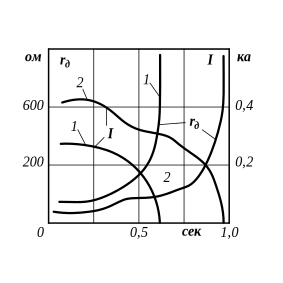
\includegraphics[width=0.5\linewidth]{1-1}
	\caption{}
	\label{fig:q}
\end{wrapfigure}

\begin{figure}
\centering
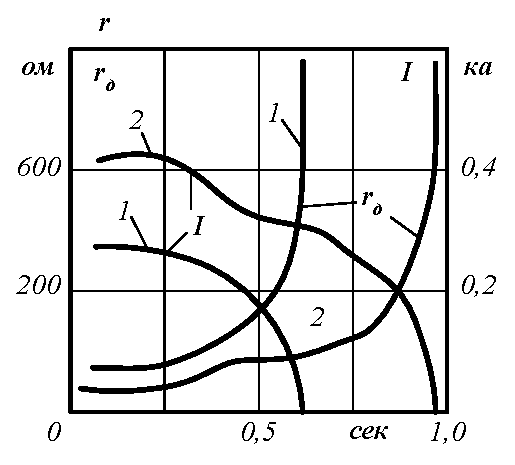
\includegraphics[width=0.7\linewidth]{a}
\caption{}
\label{fig:a}
\end{figure}


Когда токи достаточно велики (сотни ампер и более), сопротивление дуги приблизительно постоянно и по
своему характеру почти чисто активное. С уменьшением, тока и увеличением длины дуги, что имеет место в течение переходного процесса, ее сопротивление возрастает. Наглядной иллюстрацией такого изменения могут служить графики (рис. 1-1), полученные экспериментально при возникновении самопогасающих дуг на линиях
110~\textit{кв} с деревянными опорами.







\chapter{Общие указания к выполнению расчетов}

\section{Основные допущения}

Как отмечалось выше, расчет электромагнитного переходного процесса в современной электрической системе с учетом всех имеющих место условий и факторов чрезвычайно сложен и практически невыполним. Поэтому, чтобы упростить задачу и сделать ее решение практически возможным, вводят ряд допущений. Последние зависят прежде всего от характера и постановки самой задачи. Те допущения, которые вполне пригодны при решении одной задачи, могут быть совершенно неприемлемыми при решении другой.

Каждый из практических методов расчета, электромагнитных переходных процессов, в частности процесса при коротком замыкании, основан на некоторых допущениях, касающихся преимущественно возможности использование упрощённых представлений об изменении свободных токов в сложных схемах с несколькими источниками, о разных способах учета автоматического регулирования возбуждения синхронных машин и т.~п. C ними читатель познакомится в ходе дальнейшего изложения материала. Здесь же остановимся только на тех основных допущениях, которые обычно принимают при решении большинства практических задач, связанных с определением токов и напряжений при электромагнитных переходных процессах. К  числу таких допущений следует отнести:

\begin{enumerate} 
	\item
	отсутствие насыщения магнитных систем. При этом все схемы оказываются линейными, расчет которых значительно проще; в частности, здесь могут быть использованны любые формы принципа наложения.
	\item
	Пренебрежение токами намагничивания трансформаторов и автотрансформаторов. Единственным исключением их этого допущения является случай, когда трехстержневой трансформатор с соединением обмоток $ Y_{0}/Y_{0} $ включен на напряжение нулевой последовательности (см.~\colorbox{red}{§12-5}).
	\item
	Сохранение симметрии трехфазное системы. Оня нарушается обычно лишь для какого-либо одного элемента, что происходит в результату его повреждения, или преднамеренно по специальным соображениям (см. гл.~\colorbox{red}{15}).
	\item
	Пренебрежение емкостными проводимостями. Это допущение обычно является, уместным и заметно не искажает результаты решения, если в рассматриваемой схеме нет продольной компенсации индуктивности цепи, а также дальних линий передач напряжением выше 220~\textit{кв}. При рассмотрении простых замыканий на землю (см.~§\colorbox{red}{17-2}) это допущение, разумеется, совсем непригодно, так как в данном случае ток замыкается именно через емкостные проводимости.
	\item
	Приближенный учет нагрузок. В зависимости от стадии переходного процесса нагрузку приближенно характеризуют некоторым постоянным сопротивлением, обычно чисто индуктивным (см.~\colorbox{red}{§5-4 и §6-5}).
	\item
	Отсутствие активных сопротивлений. Это допущение в известной мере условно. Оно приемлемо при определении начальных и конечных значений отдельных величин, характеризующих переходный процесс в основных звеньях высокого напряжения электрической системы; при этом приближенный учет активных сопротивлений находит отражение при оценке постоянных времени затухания свободных составляющих рассматриваемых величин. В тех же случаях, когда подобный расчет проводится для протяженной кабельной или воздушной сети с относительно небольшими сечениями проводников (особенно линии со стальными проводами), а также для для установок и сетей напряжением до 1~\textit{кв}, данное допущение непригодно (см.~\colorbox{red}{гл. 17}).
	\item
	Отсутствие качаний синхронных машин. Если задача ограничена рассмотрением лишь начальной стадии переходного процесса (т.~е. в пределах 0,1--0,2~\textit{сек} с момента нарушения режима до отключения повреждения), это допущение обычно не вносит заметной погрешности (особенно в токе в месте повреждения). Однако при возникновении существенных качаний или выпадении машин из синхронизма достаточно надежный результат может быть получен лишь с учетом (хотя бы приближенным) такого процесса (см.~\colorbox{red}{гл. 19}).
\end{enumerate}

\section{Понятие о расчетных условиях}

В соответствии с целевым назначением проводимого на практике расчета электромагнитного переходного процесса устанавливают исходные расчетные условия. Они весьма разнообразны и при решении разных задач могут быть даже противоположными.

Так, например, для выбора выключателя по условиям его работы при коротком замыкании должны быть определены соответствующие возможные наибольшие величины тока короткого замыкания. С этой целью исходят из предположения, что короткое замыкание происходит в то время, когда включено наибольшее число генераторов, что вид короткого замыкания такой, при котором ток достигает наибольшей величины, что короткое замыкание металлическое и что оно произошло непосредственно у выводов самого выключателя. Помимо того, здесь устанавливают расчетное время размыкания контактов выключателя и цикл производимых им операций (включение и отключение).

Для выбора трубчатого разрядника требуется знать не только наибольшую, но и возможную наименьшую величину тока короткого замыкания, для определения которой, разумеется, должны быть приняты совсем иные расчетные условия.

Большое разнообразие расчетных условий встречается при выполнении расчетов для выбора и настройки устройств релейной защиты и автоматики. В них устанавливаются исходные предшествующие режимы заданной системы, число и расположение заземленных нейтралей, виды повреждений, и последовательность отключения поврежденного участка и т.~п.

При решении вопроса гашения поля синхронной машины в качестве расчетного режима может быть как режим короткого замыкания, так и холостого хода.

Приведенные примеры показывают, сколь велико разнообразие расчетных условий. Обоснование расчетных условий для конкретных технических задач (с учетом вероятности отдельных факторов) является одним из важных вопросов соответствующих специальных дисциплин.

\section{Система относительных единиц}

Представление любых физических величин не в обычных для них соответствующих именованных единицах, а в относительных, безразмерных единицах позволяет существенно упростить некоторые теоретические выкладки и придать им более общий характер. Равным образом и в практических расчетах такое представление величин придает результатам большую наглядность и позволяет быстрее ориентироваться в порядке определяемых значений. Благодаря этому система относительных единиц широко используется, хотя на первый взгляд она может казаться несколько искусственной и даже излишней.

С выражением величин в относительных единицах (в долях или процентах) читатель уже встречался при изучении электрических машин, где реактивности обычно выражают в долях единицы, напряжения короткого замыкания трансформаторов --- в процентах, пусковые токи и моменты асинхронных двигателей --- в кратностях от их номинальных значений и т.~д. Теперь нам нужно познакомиться с системой относительных единиц в более широком аспекте, имея в виду использование ее при решении различных вопросов и задач для схем с произвольным числом всевозможных элементов.

Напомним, что под относительным значением какой-либо величины следует понимать ее отношение к другой одноименной величине, выбранной за единицу измерения. Следовательно, чтобы выразить отдельные величины в относительных единицах, нужно прежде всего выбрать те величины, которые должны служить соответственными единицами измерения, или, как говорят, установить базисные единицы (или условия).

Пусть за базисный ток и базисное междуфазное напряжение приняты некоторые произвольные величины $ I_{\mbox{б}} $ и $ U_{\mbox{б}} $. Тогда базисная мощность трехфазной системы, очевидно, будет:

\begin{equation}
	\label{eq:chap2 S_baz}
	S_{\mbox{б}} = \sqrt{3}U_{\mbox{б}}I_{\mbox{б}}
\end{equation}

и базисное сопротивление

\begin{equation}
	\label{eq:chap2 z_baz}
	z_{\mbox{б}} = \frac{U_{\mbox{б}}}{\sqrt{3}I_{\mbox{б}}}
\end{equation}

т.~е. оно подчинено закону Ома, чтобы обеспечить тождественную запись этого закона как в именованных, так и в относительных единицах.

Как видно, из четырех базисных единиц $ I_{\mbox{б}} $, $ U_{\mbox{б}} $, $ S_{\mbox{б}} $ и $ z_{\mbox{б}} $ только две могут быть выбраны произвольно, а две другие уже получаются из указанных соотношений. Фазные и междуфазные базисные напряжения, а также фазные и линейные базисные токи связаны между собой известными соотношениями для симметричной трехфазной системы. Следует особо подчеркнуть, что выбранные базисные единицы служат для, измерения как полных величин, так и их составляющих (активных, реактивных и~пр.).

Таким образом, при выбранных базисных условиях относительные значения э.~д.~с., напряжения, тока, мощности и сопротивления будут:

\begin{equation}
	\label{eq:E_baz_otn}
	\underset{*}{E_{\mbox{б}}} = \frac{E}{U_{\mbox{б}}}
\end{equation}










%TODO: Раздел второй - ЭЛЕКТРОМАГНИТНЫЕ ПЕРЕХОДНЫЕ ПРОЦЕССЫ ПРИ СОХРАНЕНИИ СИММЕТРИИ ТРЕХФАЗНОЙ ЦЕПИ
\chapter{Переходный процесс в простейших трехфазных цепях}
\label{chap:3 perehodnyi_protcess_v_prosteishikh_trekhfaznykh_tcepiakh}

\section{Постановка задачи и ее ограничения}
\label{sec:3-1 postanovka_zadachi_i_ee_ogranicheniia}

Симметричную трехфазную цепь с сосредоточенными активными сопротивлениями и индуктивностями при отсутствии в ней трансформаторных связей условимся называть \so{простейшей} трехфазной цепью.

Электромагнитный переходный процесс в такой цепи рассмотрим сначала при условии, что ее питание осуществляется от источника, сопротивление которого равно нулю и его напряжение, изменяясь с постоянной частотой, имеет неизменную амплитуду\footnote{Применение чувствительного и быстродействующего автоматического регулировании возбуждения генераторов дополнительно способствует принятию указанного предположения.}. Обычно его называют источником бесконечной  мощности.

Включение в схему такого источника, вообще говоря, соответствует теоретическому пределу, когда изменение внешних условий не влияет на работу самого источнику. Практически это имеет место, например, при коротких замыканиях в относительно маломощных электрических установках или протяженных сетях, питаемых от крупных энергетических систем (см.~\colorbox{red}{гл. 17}).

С исследованием переходных процессов в подобных условиях читатель знаком из курса теоретических основ электротехники. Поэтому задачей данной главы является кратко напомнить основные выводы такого исследования, отметить особенности многофазной цепи по сравнению с однофазной, привести некоторые упрощенные приемы расчета и обратить внимание на влияние ряда факторов.

\section{Трехфазное короткое замыкание в неразветвленной цепи}
\label{sec:3-2 trekhfaznoe_korotkoe_zamykanie_v_nerazvetvlennoi_tcepi}

Обратимся к рис.~\ref{ris:3-1 simple_3_phase_circut}, на котором представлена простейшая симметричная трехфазная цепь. В ней условно принято, что на одном ее участке имеется взаимоиндукция между фазами, а на другом она отсутствует. Цепь присоединена к источнику синусоидального напряжения с неизменными амплитудой и частотой.

Рассмотрим переходный процесс, вызванный включением выключателя \textit{B}, за которым сделана закоротка, что равносильно возникновению металлического трехфазного короткого замыкания между двумя участками данной цепи.

\begin{figure}[h]
	\center{\includegraphics[width=0.9\linewidth]{pic/3-1}}
	\caption{Простейшая трехфазная электрическая цепь.}
	\label{ris:3-1 simple_3_phase_circut}
\end{figure}

Пусть векторы $ \overset{\;.}{U}_A $, $ \overset{\;.}{U}_B $, $ \overset{\;.}{U}_C $, $ \overset{\;.}{I}_A $, $ \overset{\;.}{U}_B $, $ \overset{\;.}{U}_C $ (рис.~\ref{ris:3-2 diagram})
характеризуют предшествующий режим рассматриваемой цепи, а вертикаль \textit{tt} является неподвижной линией времени, т.~е. мгновенные значения отдельных величии определяются проекциями на эту линию соответствующих вращающихся векторов. Момент возникновения короткого замыкания будем фиксировать значением угла $ \alpha $ (т.~е. \so{фазой включения}) между вектором напряжения фазы \textit{A} и горизонталью. (рис.~\ref{ris:3-2 diagram}.

После включения выключателя \textit{В} цепь рис.~\ref{ris:3-1 simple_3_phase_circut} распадается на два независимых друг от друга участка. Участок с $ r_1 $ и $ L_1 $ оказывается зашунтированным коротким замыканием и ток в нем будет поддерживаться лишь до тех пор, пока запасенная в индуктивности $ L_1 $ энергия магнитного потока не перейдет в тепло, поглощаемое активным сопротивлением $ r_1 $.

Дифференциальное уравнение равновесия в каждой фазе этого участка имеет вид:

\begin{equation}
	0 = ir_1 + L_1 \frac{di}{dt}.
	\label{eq:3-1 diff_ur}
\end{equation}

Его решение общеизвестно:

\begin{equation}
	i = i_0 e^{-t / T_{\text{а}1}}; %TODO: Проверить формулу, какая-то черка в степени
	\label{eq:3-2 diff_solve}
\end{equation}

оно показывает, что здесь имеется лишь свободный ток, который затухает по экспоненте с постоянной времени

\begin{equation}
	T_{\text{а}1} = \frac{L_1}{r_1} = \frac{x_1}{\omega r_1}, \textit{~сек}.
	\label{eq:3-3 T_a1}
\end{equation}

Начальное значение свободного тока в каждой фазе зашунтированного участка цепи, очевидно, равно предшествовавшему мгновенному значению тока, поскольку в цепи с индуктивностью не может произойти внезапного (скачком) изменения тока. В общем случае свободные токи в фазах различны, хотя их затухание, разумеется, происходит с одной и той же постоянной времени. В одной из фаз свободный ток может вообще отсутствовать, если в момент возникновения короткого замыкания предшествовавший ток в этой фазе проходил через нуль; при этом свободные токи в двух других фазах будут одинаковы по величине, но противоположны по направлению.

На рис.~\ref{ris:3-3} слева приведены кривые изменения фазных токов в зашунтированном участке рассматриваемой цени, с учетам, что короткое замыкание произошло в момент, отвечающий положению векторов на рис.~\ref{ris:3-2 diagram}.

\begin{floatingfigure}[lflt]{0.45\linewidth}
	\centering
	\includegraphics[width=0.40\linewidth]{pic/3-2}
	\caption{Векторная диаграмма для начального момента трехфазного короткого замыкания.}
	\label{ris:3-2 diagram}
\end{floatingfigure}

\begin{small}
	Напомним, что подкасательная в любой точке экспоненты\footnote{Обычно используют начальную часть экспоненты, где скорость изменения соответствующей величины больше и поэтому можно точнее провести касательную.} в принятом для оси времени масштабе дает значение постоянной времени, с которой происходит изменение экспоненты (рис.~\ref{ris:3-3}). Имея в виду, что при $ t = T_{\text{а}} $ значение $ e^{-1} = 0,368 $, постоянную $ T_{\text{а}} $ обычно трактуют как время, в течение которого переменная величина снижается до 0,368 своего начального значения; при этом за начальную может быть принята любая точка кривой.
	
\end{small}

%TODO: Рисунок оказывается перед 3-2 ??!!
\begin{figure}
	\center{\includegraphics[width=0.85\linewidth]{pic/3-3}}
	\caption{Осциллограммы токов в фазах при внезапном трехфазном коротком замыкании в простейшей электрической цепи.}
	\label{ris:3-3}
\end{figure}

Перейдем теперь к участку цепи, который остался присоединенным к источнику. Здесь помимо свободного тока будет новый принужденный ток, величина которого, очевидно, больше предыдущего и сдвиг по фазе которого в общем случае иной. Допустим, что векторы $ I_{\text{П}A} $, $ I_{\text{П}B} $, $ I_{\text{П}C} $ (рис.~\ref{ris:3-2 diagram}) отвечают новому установившемуся режиму данного участка цепи.

Дифференциальное уравнение равновесия для любом фазы, например фазы \textit{А}, этого участка

\begin{equation*}
	u_A = i_A r_{\text{К}} + L \frac{di_A}{dt} + M \frac{di_B}{dt} + M \frac{di_C}{dt},
\end{equation*}

имея ввиду, что $ (i_B + i_C) = -i_A $, можно представить (опуская индекс фазы) как

\begin{equation}	
	u = i r_{\text{К}} + L_{\text{К}} \frac{di}{dt},
	\tag{\ref*{eq:3-1 diff_ur}а}
	\label{eq:3-1a u}
\end{equation}

где $ L_{\text{К}} = (L - M) $ --- результирующая индуктивность фазы, т.~е. индуктивность с учетом влияния двух других фаз.

Решение (\ref{eq:3-1a u}) имеет вид:

\begin{equation}	
	i = \frac{U_m}{z_{\text{К}}} sin(\omega t + \alpha - \varphi_{\text{К}}) + i_{\text{а} | 0 |} e^{-t / T_{\text{а}}}
	\tag{\ref*{eq:3-2 diff_solve}а}
	\label{eq:3-2a i}
\end{equation}

где $ z_{\text{К}} $ --- полное сопротивление присоединенного к источнику участка цепи или. короче, цепи короткого замыкания;

$ \varphi_{\text{К}} $ --- угол сдвига тока в этой цепи;
	
$ T_{\text{a}} $ --- постоянная времени цепи короткого замыкания, определяемая по (\ref{eq:3-3 T_a1}), где вместо $ L_1 $, $ x_1 $, $ r_1 $ следует ввести $ L_{\text{К}} $, $ x_{\text{К}} $, $ r_{\text{К}} $.

Первый член правой части (\ref{eq:3-2a i}) представляет периодическую слагающую тока, которая при рассматриваемых условиях является принужденным током с постоянной амплитудой $ I_{\text{П}m} = U_m / z_{\text{К}} $. Соответственно второй член представляет, как и раньше, затухающий по экспоненте свободный ток; его называют также апериодической слагающей тока. Начальное значение этой слагающей определяется из начальных условий, т.~е.

% В этом месте в книге опечатка, формула названа 3-3, нумерация дальше отличается
\begin{equation}
	i_0 = i_{\text{п}~/0/} + i_{\text{а}~/0/},
	\label{eq:3-4 i_0}
\end{equation}

откуда после подстановки соответствующих выражений имеем:

\begin{equation}
	i_{\text{а}|0|} = I_m sin(\alpha - \varphi) - I_{\text{П}m} sin(\alpha - \varphi_{\text{К}}).
	\label{eq:3-5 i_a0}
\end{equation}

Поскольку токи $ i_{\text{П}} $, $ i_0 $ являются проекциями векторов $ \overset{\;.}{I}_{\text{П}m} $ и $ \overset{\;.}{I}_m $ на линию времени, то ток $ 	i_{\text{а}|0|} $ также можно рассматривать как проекцию вектора $ (\overset{\;.}{I}_m - \overset{\;.}{I}_{\text{П}m} $ на ту же линию (рис.~\ref{ris:3-2 diagram}). В зависимости от фазы включения $ \alpha $ начальное значение тока $ 	i_{\text{а}|0|} $ может изменяться от возможной наибольшей величины, когда вектор $ (\overset{\;.}{I}_m - \overset{\;.}{I}_{\text{П}m} $ параллелен линии времени, до нуля, когда этот вектор нормален к ней. В трехфазной системе такие частные условия, разумеется, могут быть лишь в одной из фаз.

\begin{figure}
	\center{\includegraphics[width=0.85\linewidth]{pic/3-4}}
	\caption{Осциллограмма тока короткого замыкания при наибольшей апериодической слагающей.}
	\label{ris:3-4}
\end{figure}

На рис.~\ref{ris:3-3} справа представлены кривые изменения токов в фазах рассматриваемого участка при трехфазном коротком замыкании. Как видно, чем больше апериодическая слагающая тока, тем больше смещение кривой полного тока относительно оси времени. Эту слагающую можно рассматривать как криволинейную ось симметрии кривой полного тока, из которой ее легко выделить. Для этого нужно сначала провести огибающие по максимальным положительным и отрицательным значениям заданной кривой тока (см. пунктирные линии у кривой тока фазы \textit{А} на рис.~\ref{ris:3-3}). Каждая точка кривой апериодической слагающей лежит посредине вертикального отрезка между этими огибающими.

Из (\ref{ris:3-4}) и рис.~\ref{ris:3-2 diagram} следует, что наибольшее значение апериодической слагающей тока определяется не только фазой включения, но также предшествующим режимом цепи. Так, например, при отсутствии предшествующего тока в данной цепи величина 
при отсутствии величина $ i_{\text{а}/0/} $ может достигать амплитуды периодической слагающей, если в момент короткого замыкания эта слагающая проходит через свой положительный или отрицательный максимум (рис.~\ref{ris:3-4}). Обычно этот случай рассматривается как расчетный\footnote{Хотя возможны частные случаи, когда начальное значение апериодической слагающей тока превышает амплитуду периодической слагающей.}.

Важно отметить, что фаза включения, при которой возникает наибольшее значение апериодической слагающей, еще не предопределяет того, что именно при ней будет максимум мгновенного значения полного тока. В самом деле, из (\ref{eq:3-2a i}) и (\ref{eq:3-5 i_a0}) при отсутствии предшествующего тока ($ I_m = 0 $) следует, что полный ток в цепи короткого замыкания является функцией двух независимых переменных: времени $ t $ и фазы включения $ \alpha $ и выражается уравнением

\begin{equation}
	i = I_{\text{п}m} [sin( \omega t + \alpha - \varphi_{\text{к}}) - sin(\alpha - \varphi_{\text{к}}) e^{-t/T_{\text{a}}} ].
	\label{eq:3-6 i}
\end{equation}

%TODO: не пропущена ли здесь буква "к"
Приравняв к нулю частные производные этого уравнения, т.~е.

\begin{equation*}
	\frac{di}{dt} = \omega cos( \omega t + \alpha - \varphi_{\text{к}} ) + \frac{1}{T_{\text{a}}} sin( \alpha - \varphi_{\text{к}} ) e^{-t/T_{\text{a}}} = 0;
\end{equation*}

\begin{equation*}
	\frac{di}{d \alpha} = cos( \omega t + \alpha - \varphi_{\text{к}} ) - cos( \alpha - \varphi_{\text{к}} ) e^{-t/T_{\text{a}}} = 0,
\end{equation*}

и совместно решив эти уравнения, найдем, что максимум тока наступает при

\begin{equation*}
	tg( \alpha - \varphi_{\text{к}} ) = -\omega T_{\text{a}} = - \frac{x_{\text{к}}}{r_{\text{к}}} = tg( -\varphi_{\text{к}}).
\end{equation*}

т.~е. при $ \alpha = 0 $.

Следовательно, в предварительно разомкнутой цепи с $ r $ и $ L $ максимум мгновенного значения полного тока при коротком замыкании наступает, если в момент возникновения короткого
%TODO: пропущено слово "замыкания"
замыкания напряжение источника проходит через нуль.

Для цепей с преобладающей индуктивностью $ \varphi_{\text{к}} \approx 90^\circ $. поэтому условие возникновения наибольшей апериодической слагающей и условие, при котором достигается максимум мгновенного значения полного тока очень близки друг к другу. Поэтому в практических расчетах максимальное мгновенное значение полного тока короткого замыкания, которое называют \so{ударным током короткого замыкания $ i_{\text{у}} $},   обычно находят при наибольшем значении апериодической слагающей (рис.~\ref{ris:3-4}), считая, что он наступает приблизительно через полпериода, что при $ f = 50 \textit{~гц} $ составляет около 0,01~\textit{сек} с возникновения короткого замыкания.

Таким образом, выражение для ударного тока короткого замыкания можно записать в следующем виде:

\begin{equation}
	i_{\text{у}} = I_{\text{п}m} + I_{\text{п}m} e^{-0,01 / T_{\text{а}}} = k_{\text{у}} I_{\text{п}m},
	\label{eq:3-7 i_y}
\end{equation}

где

\begin{equation}
	k_{\text{у}} = 1 + e^{-0,01 / T_{\text{а}}},
	\label{eq:3-8 k_y}
\end{equation}

который называют \so{ударным коэффициентом}, показывает превышение ударного тока над амплитудой периодической слагающей; его величина находится в пределах

\begin{equation*}
	1 < k_{\text{у}} < 2,
\end{equation*}

что соответствует предельным значениям $ T_{\text{а}} $, т.~е. $ T_{\text{а}} = 0 $ (при $ L_{\text{к}} = 0 $)  и $ T_{\text{а}} = \infty $ (при $ r_{\text{к}} = 0 $).

Естественно, чем меньше $ T_{\text{а}} $, тем быстрее затухает апериодическая слагающая и тем соответственно меньше ударный коэффициент. Влияние этой слагающей сказывается лишь в начальной стадии переходного процесса; в сетях и установках высокого напряжения она практически исчезает спустя 0,1--0,3~\textit{сек}, а в установках низкого напряжения она практически совсем незаметна.

Еще раз подчеркнем, что апериодические слагающие токов в фазах различны. Поэтому определение трехфазного короткого замыкания как симметричного, строго говоря, справедливо применительно к периодическим слагающим фазных токов.








\bibliographystyle{unsrt} % сортировка литературы в порядке упоминания (не как в книге)
\bibliography{./tex/lit}
\addcontentsline{toc}{chapter}{\bibname}

\backmatter
% bibliography, glossary and index would go here.

\end{document}